\documentclass{standalone}
\usepackage{tikz}
\usetikzlibrary{patterns, positioning}
\usetikzlibrary{shapes.misc}
\usepackage[outline]{contour}
\contourlength{1.5pt} 
\usepackage[sfdefault]{ClearSans} %% option 'sfdefault' activates Clear Sans as the default text font
\usepackage[T1]{fontenc}

\begin{document}
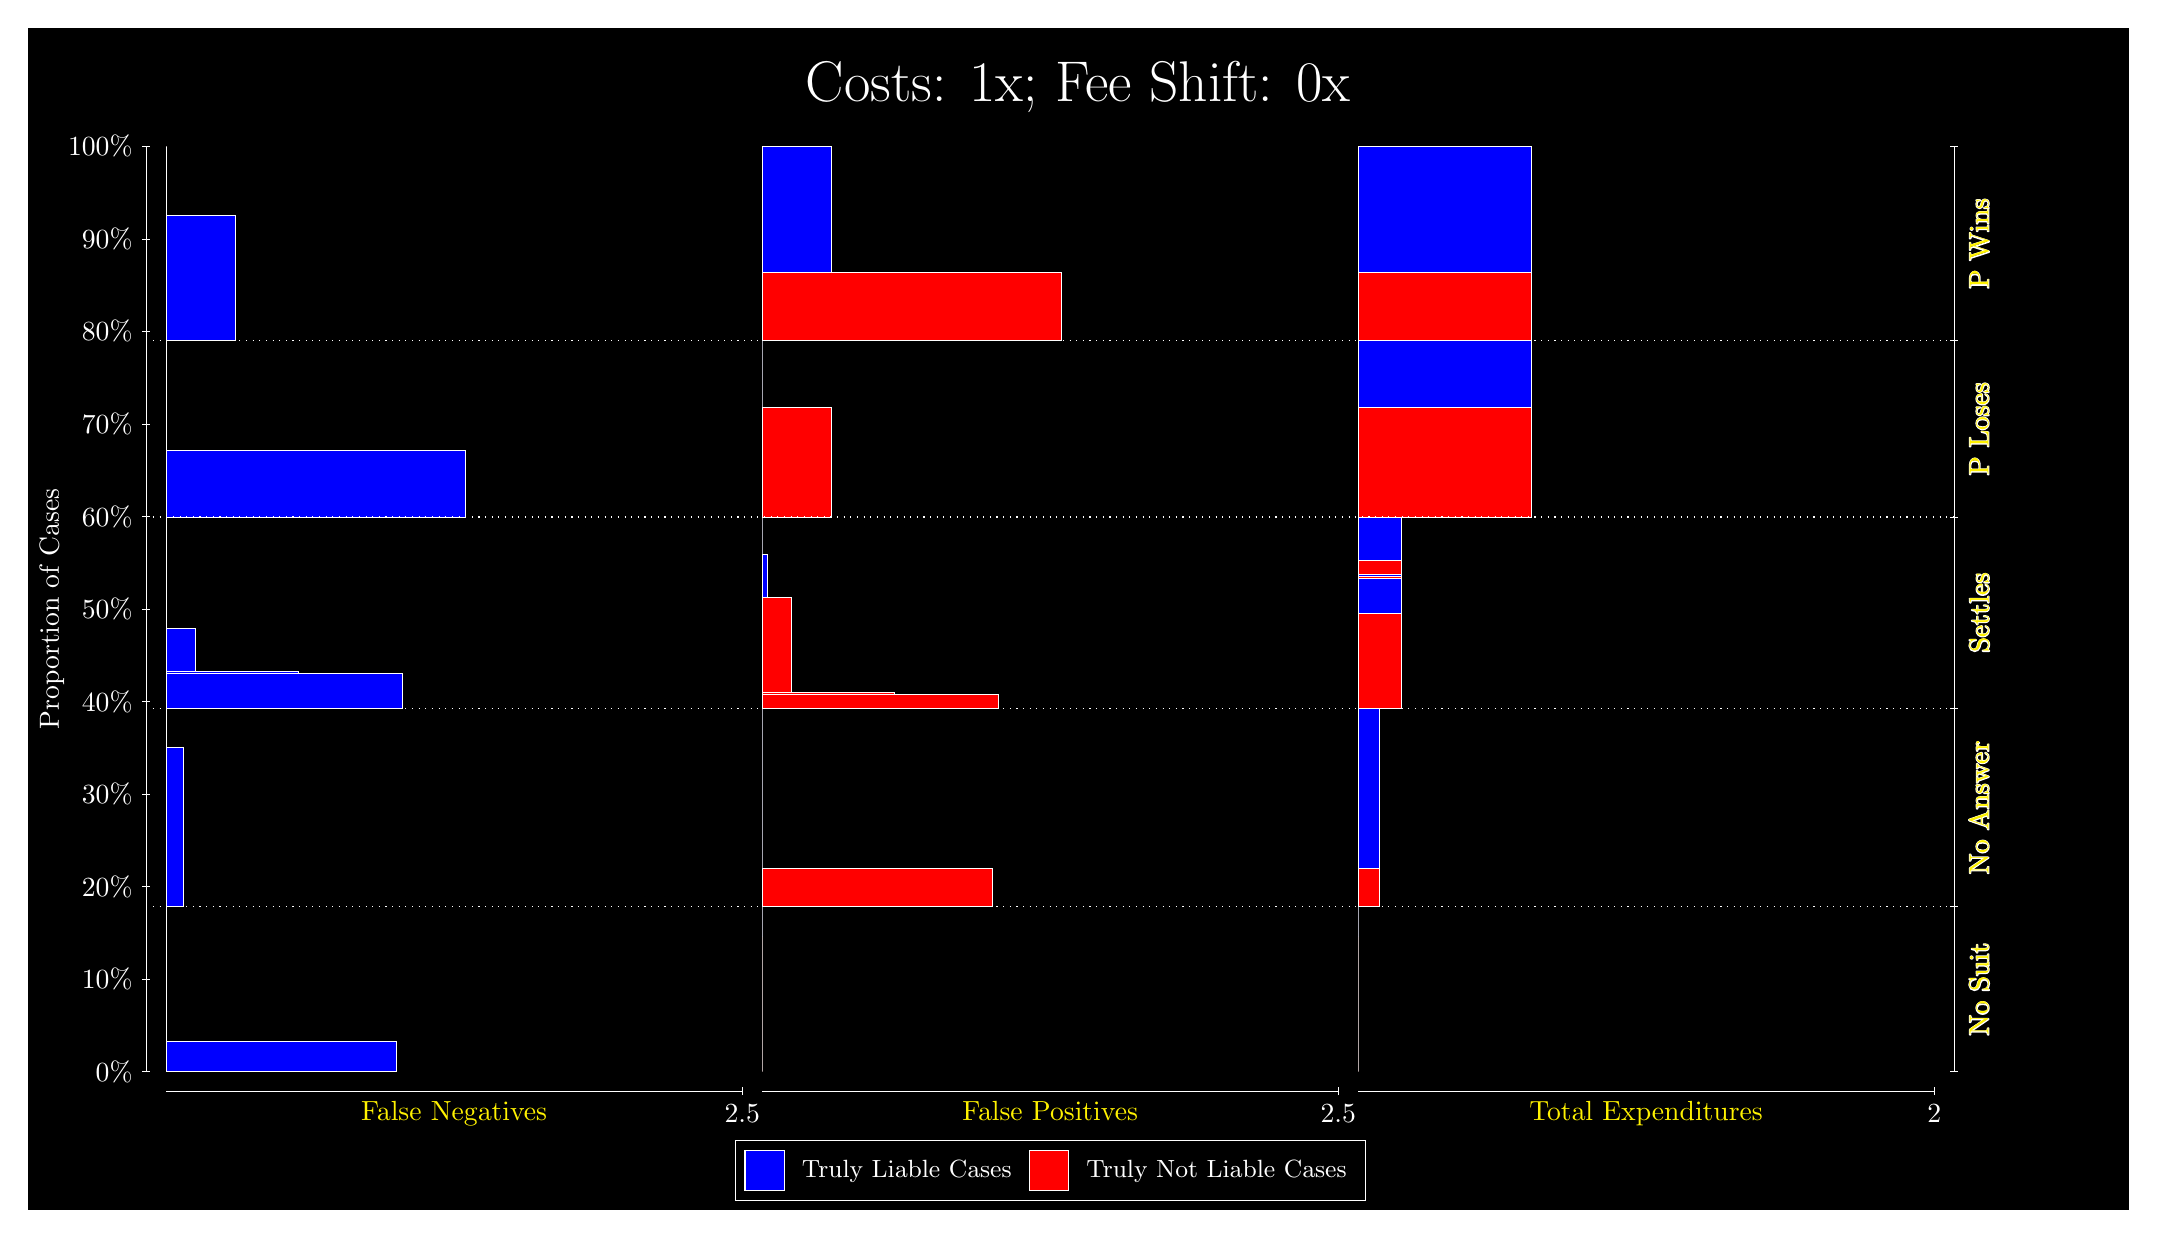
\begin{tikzpicture}
\draw[fill=black] (0,0) rectangle (26.667,15);
\draw[text=white] (0,13.5) rectangle (26.667,15) node[midway] {\huge Costs: 1x; Fee Shift: 0x};
\draw[white, very thin] (1.5,1.75) -- (1.5,13.5);
\node[rotate=90, text=white, anchor=center] at (0.3, 7.625) {Proportion of Cases};
\draw[white, very thin] (1.45,1.75) -- (1.55,1.75);
\node[text=white, anchor=east] at (1.45, 1.75) {0\%};
\draw[white, very thin] (1.45,2.925) -- (1.55,2.925);
\node[text=white, anchor=east] at (1.45, 2.925) {10\%};
\draw[white, very thin] (1.45,4.1) -- (1.55,4.1);
\node[text=white, anchor=east] at (1.45, 4.1) {20\%};
\draw[white, very thin] (1.45,5.275) -- (1.55,5.275);
\node[text=white, anchor=east] at (1.45, 5.275) {30\%};
\draw[white, very thin] (1.45,6.45) -- (1.55,6.45);
\node[text=white, anchor=east] at (1.45, 6.45) {40\%};
\draw[white, very thin] (1.45,7.625) -- (1.55,7.625);
\node[text=white, anchor=east] at (1.45, 7.625) {50\%};
\draw[white, very thin] (1.45,8.8) -- (1.55,8.8);
\node[text=white, anchor=east] at (1.45, 8.8) {60\%};
\draw[white, very thin] (1.45,9.975) -- (1.55,9.975);
\node[text=white, anchor=east] at (1.45, 9.975) {70\%};
\draw[white, very thin] (1.45,11.15) -- (1.55,11.15);
\node[text=white, anchor=east] at (1.45, 11.15) {80\%};
\draw[white, very thin] (1.45,12.325) -- (1.55,12.325);
\node[text=white, anchor=east] at (1.45, 12.325) {90\%};
\draw[white, very thin] (1.45,13.5) -- (1.55,13.5);
\node[text=white, anchor=east] at (1.45, 13.5) {100\%};

\draw[white, very thin] (24.457,1.75) -- (24.457,13.5);
\draw[white, very thin] (24.407,1.75) -- (24.507,1.75);
\node[anchor=west] at (24.407, 1.75) {};
\draw[white, very thin] (24.407,3.843) -- (24.507,3.843);
\node[anchor=west] at (24.407, 3.843) {};
\draw[white, very thin] (24.407,6.3605) -- (24.507,6.3605);
\node[anchor=west] at (24.407, 6.3605) {};
\draw[white, very thin] (24.407,8.7924) -- (24.507,8.7924);
\node[anchor=west] at (24.407, 8.7924) {};
\draw[white, very thin] (24.407,11.031) -- (24.507,11.031);
\node[anchor=west] at (24.407, 11.031) {};
\draw[white, very thin] (24.407,13.5) -- (24.507,13.5);
\node[anchor=west] at (24.407, 13.5) {};

\draw[white, very thin, fill=blue] (1.75,1.75) rectangle (4.6775,2.1326);
\draw[white, very thin, fill=red] (1.75,2.1326) rectangle (1.75,3.843);
\draw[white, very thin, fill=blue] (1.75,3.843) rectangle (1.9696,5.8718);
\draw[white, very thin, fill=red] (1.75,5.8718) rectangle (1.75,6.3605);
\draw[white, very thin, fill=blue] (1.75,6.3605) rectangle (4.7507,6.8111);
\draw[white, very thin, fill=blue] (1.75,6.8111) rectangle (3.4333,6.8337);
\draw[white, very thin, fill=blue] (1.75,6.8337) rectangle (2.1159,7.3853);
\draw[white, very thin, fill=red] (1.75,7.3853) rectangle (1.75,8.7924);
\draw[white, very thin, fill=blue] (1.75,8.7924) rectangle (5.5558,9.6341);
\draw[white, very thin, fill=red] (1.75,9.6341) rectangle (1.75,11.031);
\draw[white, very thin, fill=blue] (1.75,11.031) rectangle (2.6283,12.628);
\draw[white, very thin, fill=red] (1.75,12.628) rectangle (1.75,13.5);
\draw[white, very thin, fill=red] (9.3189,1.75) rectangle (9.3189,3.4605);
\draw[white, very thin, fill=blue] (9.3189,3.4605) rectangle (9.3189,3.843);
\draw[white, very thin, fill=red] (9.3189,3.843) rectangle (12.246,4.3318);
\draw[white, very thin, fill=blue] (9.3189,4.3318) rectangle (9.3189,6.3605);
\draw[white, very thin, fill=red] (9.3189,6.3605) rectangle (12.32,6.5418);
\draw[white, very thin, fill=red] (9.3189,6.5418) rectangle (11.002,6.5623);
\draw[white, very thin, fill=red] (9.3189,6.5623) rectangle (9.6848,7.7675);
\draw[white, very thin, fill=blue] (9.3189,7.7675) rectangle (9.3921,8.3191);
\draw[white, very thin, fill=blue] (9.3189,8.3191) rectangle (9.3189,8.7924);
\draw[white, very thin, fill=red] (9.3189,8.7924) rectangle (10.197,10.189);
\draw[white, very thin, fill=blue] (9.3189,10.189) rectangle (9.3189,11.031);
\draw[white, very thin, fill=red] (9.3189,11.031) rectangle (13.125,11.903);
\draw[white, very thin, fill=blue] (9.3189,11.903) rectangle (10.197,13.5);
\draw[white, very thin, fill=red] (16.888,1.75) rectangle (16.888,3.4605);
\draw[white, very thin, fill=blue] (16.888,3.4605) rectangle (16.888,3.843);
\draw[white, very thin, fill=red] (16.888,3.843) rectangle (17.162,4.3318);
\draw[white, very thin, fill=blue] (16.888,4.3318) rectangle (17.162,6.3605);
\draw[white, very thin, fill=red] (16.888,6.3605) rectangle (17.437,7.5658);
\draw[white, very thin, fill=blue] (16.888,7.5658) rectangle (17.437,8.0163);
\draw[white, very thin, fill=red] (16.888,8.0163) rectangle (17.437,8.0368);
\draw[white, very thin, fill=blue] (16.888,8.0368) rectangle (17.437,8.0595);
\draw[white, very thin, fill=red] (16.888,8.0595) rectangle (17.437,8.2408);
\draw[white, very thin, fill=blue] (16.888,8.2408) rectangle (17.437,8.7924);
\draw[white, very thin, fill=red] (16.888,8.7924) rectangle (19.083,10.189);
\draw[white, very thin, fill=blue] (16.888,10.189) rectangle (19.083,11.031);
\draw[white, very thin, fill=red] (16.888,11.031) rectangle (19.083,11.903);
\draw[white, very thin, fill=blue] (16.888,11.903) rectangle (19.083,13.5);
\draw[white, dotted] (1.5,3.843) -- (24.457,3.843);
\draw[white, dotted] (1.5,6.3605) -- (24.457,6.3605);
\draw[white, dotted] (1.5,8.7924) -- (24.457,8.7924);
\draw[white, dotted] (1.5,11.031) -- (24.457,11.031);
\draw[white, very thin] (1.75,1.5) -- (9.0689,1.5);
\node[text=yellow, anchor=north] at (5.4094, 1.5) {False Negatives};
\draw[white, very thin] (9.0689,1.45) -- (9.0689,1.55);
\node[text=white, anchor=north] at (9.0689, 1.45) {2.5};

\draw[white, very thin] (9.3189,1.5) -- (16.638,1.5);
\node[text=yellow, anchor=north] at (12.978, 1.5) {False Positives};
\draw[white, very thin] (16.638,1.45) -- (16.638,1.55);
\node[text=white, anchor=north] at (16.638, 1.45) {2.5};

\draw[white, very thin] (16.888,1.5) -- (24.207,1.5);
\node[text=yellow, anchor=north] at (20.547, 1.5) {Total Expenditures};
\draw[white, very thin] (24.207,1.45) -- (24.207,1.55);
\node[text=white, anchor=north] at (24.207, 1.45) {2};

\node[text=yellow, centered, rotate=90] at (24.777, 2.7965) {\contour{white}{No Suit}};
\node[text=yellow, centered, rotate=90] at (24.777, 5.1018) {\contour{white}{No Answer}};
\node[text=yellow, centered, rotate=90] at (24.777, 7.5764) {\contour{white}{Settles}};
\node[text=yellow, centered, rotate=90] at (24.777, 9.9116) {\contour{white}{P Loses}};
\node[text=yellow, centered, rotate=90] at (24.777, 12.265) {\contour{white}{P Wins}};

\draw (12.978300999999998,1.5) node[draw=none] (baseCoordinate) {};
\begin{scope}[align=center]
        \matrix[scale=0.5, draw=white, below=0.5cm of baseCoordinate, nodes={draw}, column sep=0.1cm]{
            \node[rectangle, draw, minimum width=0.5cm, minimum height=0.5cm, fill=blue] {}; &
            \node[draw=none, font=\small, text=white] (B) {Truly Liable Cases}; &
            \node[rectangle, draw, minimum width=0.5cm, minimum height=0.5cm, fill=red] {}; &
            \node[draw=none, font=\small, text=white] (B) {Truly Not Liable Cases}; \\
            };
\end{scope}

\end{tikzpicture}
\end{document}